\graphicspath{{figures/Design/IPController/}}
\chapter{Design of the Inverted Pendulum Controller}\label{sec:IPController}
The goal of the controller is to balance the stick in an upright position. 
The system is inherently unstable as is evident by the pole in the right half plane of the pole-zero plot as seen on \autoref{fig:pzip}.

\begin{figure}[htbp]
\centering
\missingfigure{}
\caption{Pole-zero plot for the inverted pendulums transfer function.}
\label{fig:pzip}
\end{figure}
\todo[inline,author=Jacob]{Missing constants from motor test to do plot.}

There's a plethora of different options for the controller to use, the simplest being a proportional controller. A simple way to check whether the proportional controller is feasible is by examining the root locus of the transfer function in figure \autoref{fig:locusIP}. The pole in the right half plane moving towards infinity is caused by the transfer function being negative and can be fixed with a negative gain as shown on figure \autoref{fig:locusNegative}.

\begin{figure}[htbp]
\centering
\missingfigure{}
\caption{Root locus of the inverted pendulums transfer function.}
\label{fig:locusIP}
\end{figure}

\begin{figure}[htbp]
\centering
\missingfigure{}
\caption{Root locus of the inverted pendulums transfer function with a negative gain.}
\label{fig:locusNegative}
\end{figure}

The proportional controller isn't feasible as the pole in the right half plane never enters the stable region even with a negative gain.

There are two options to bring the unstable pole into the stable region: The zero in 0 can be cancelled allowing the unstable pole to cross the imaginary axis along the real axis or another pole can be added in the right half plane forcing both off the real axis with a high enough gain. The second method requires a zero in the left half plane to pull the poles towards the stable region.

Cancelling zeros in 0 by adding poles can be dangerous as the steady state error will no longer be zero which is critical for a stable inverted pendulum. The system is difficult to control as the transfer function was derived with an attempt to control the angle of the stick. This is only really possible in the special case where the reference is exactly 0 at all times. Redefining the system as trying to control the position of a point on the stick in relation to the vertical axis. By controlling the position instead of the angle would mean the system would still have to balance the stick but not be forced to use a reference of 0 at all times. This could make the system easier to control.

\section{Redefining the inverted pendulums output and reference point}

The inverted pendulum model will be redefined so the output is the distance a point on the stick to the vertical axis (where the arm and stick both have angles of 0) instead of the angle of the stick. The point, $\alpha$, and the distance to the vertical axis, $x_\alpha$, are seen on \autoref{fig:modelDist}.

\begin{figure}[htbp]
\centering
\includegraphics[width=0.7\textwidth]{ModelDist}
\caption{Diagram of the distance that will be controlled instead of the angle of the stick.}
\label{fig:modelDist}
\end{figure}

The distance to the point, $\alpha$, can be described by \autoref{eq:xa}.
\begin{flalign}\label{eq:xa}
& x_\alpha(t) = l_a\sin(\theta_a(t))+l_\alpha\sin(\theta_s(t))
\end{flalign}
This is not a linear equation and needs to be linearized in order to Laplace transform it. This is done with a 1st order Taylor approximation around the equilibrium where $\theta_a=\theta_s=0$ in \autoref{eq:xaTaylor}
\begin{subequations}\label{eq:xaTaylor}
\begin{flalign}
& x_\alpha(t)\approx l_a\sin(0)+l_a\cos(0)\theta_a(t)+l_\alpha\sin(0)+l_\alpha\cos(0)\theta_s(t) \\
& x_\alpha(t)\approx l_a\theta_a(t)+l_\alpha\theta_s(t)
\end{flalign}
\end{subequations}
This will then be Laplace transformed in \autoref{eq:xaLaplace}.
\begin{flalign}\label{eq:xaLaplace}
X_\alpha(s)=l_a\Theta_a(s)+l_\alpha\Theta_s(s) 
\end{flalign}

By isolating $\Theta_s(s)$ in \autoref{eq:tfArmStick} and inserting it into \autoref{eq:xaLaplace}, the transfer function in \eqref{eq:xatf} is found. The friction part is removed per \autoref{tab:IPModelVar}.

\begin{subequations}
\begin{flalign}
& X_\alpha(s)=l_a\Theta_a(s)+l_\alpha\frac{-\frac{3l_a}{2l_s}s^2}{s^2-\frac{3g}{2l_s}}\Theta_a(s) \\
& X_\alpha(s)=\frac{l_a\left(s^2-\frac{3g}{2l_s}\right)+l_\alpha\left(-\frac{3l_a}{2l_s}s^2\right)}{s^2-\frac{3g}{2l_s}}\Theta_a(s) \\
& \frac{X_\alpha(s)}{\Theta_a(s)} = \frac{s^2\left(l_a-l_\alpha\frac{3l_a}{2l_s}\right)-l_a\frac{3g}{2l_s}}{s^2-\frac{3g}{2l_s}} \label{eq:xatf}
\end{flalign}
\end{subequations}
The transfer function still ends up with 2 zeros but it's possible to remove them by selecting the point $\alpha$ so $l_\alpha=\frac{2l_s}{3}$. Inserting this into \autoref{eq:xatf} the transfer function becomes \autoref{eq:xaTF}.
\begin{flalign}\label{eq:xaTF}
& \frac{X_\alpha(s)}{\Theta_a(s)} = \frac{-l_a\frac{3g}{2l_s}}{s^2-\frac{3g}{2l_s}}
\end{flalign}

The zeros in 0 has now been removed but the distance, $x_\alpha$, needs to be measured. This can be done by measuring the angles which was also necessary before but now use \autoref{eq:xa} to calculate the distance instead of using the angle directly. The controller for the transfer function in \autoref{eq:xaTF} can now be designed}

\section{Design of Controller for Arm to Stick Position}



\section{Controller with a 2nd right half plane pole added}
\todo[author=Jacob, inline]{A lot of this only applies for 2nd order system which this is not. I already wrote it without considering that so this section might have to be deleted but I'm leaving it for now.}
This controller adds a zero and a pole to the system and thus have three variables that needs to be chosen: The gain and the locations of the zero and the pole. The pole has to be located somewhere in the right half plane and the zero in the left. Their locations influence the root locus of the system.

To make the system as stable as possible a fast rise time and low overshoot is desirable. From the specifications the overshoot is set as maximum 10\% with no requirements for the rise time. The damping ratio, $\zeta$, can be found from the overshoot percentage, $M_p$, by \autoref{eq:IPOvershoot}.
\begin{subequations}
\begin{flalign}
& M_p=100\exp^{\frac{-\pi\zeta}{\sqrt{1-\zeta^2}}}<10\%  \\
& \zeta = \sqrt{\frac{\left(\ln{\frac{M_p}{100}}\right)^2}{\pi^2+\left(\ln{\frac{M_p}{100}}\right)^2}}  \\
& \zeta > \sqrt{\frac{\left(\ln{\frac{10\%}{100}}\right)^2}{\pi^2+\left(\ln{\frac{10\%}{100}}\right)^2}} = 0.59 \label{eq:IPOvershoot}
\end{flalign}
\end{subequations}

The damping ratio then has to be larger than 0.59 in order to have a overshoot of less than 10\% as specified. The rise time, $t_r$, is approximated by \autoref{eq:IPRisetime}.
\begin{flalign}\label{eq:IPRisetime}
& t_r =\frac{2.2}{\zeta\omega_n} 
\end{flalign}

In order to get as fast a rise time as possible the natural frequency and damping ratio both needs to be maximized. The natural frequency can be found on the root locus by the length from the poles to the origin. The damping ratio is found by the angle from the imaginary axis to the poles. As both $\zeta$ and $\omega_n$ are dependent on the pole locations it's possible that the fastest response time comes with a damping ratio below 0.59. The goal of this controller is to minimize \autoref{eq:IPRisetime} but maintaining a damping ratio above 0.59.

The location of the pole, and zero and the gain can thus be decided in order to achieve final pole locations with as far away from the origin as possible while having an angle to the imaginary axis that corresponds to $\zeta=0.59$.

%For the inverted pendulum it's also worth to consider a controller that keeps the arm at zero radians as well as it has a much harder time controlling the arm when out of the upright position. Therefore two controllers will be made: A single-input single-output (SISO) controller that only controls the angle of the stick and a single-input multiple-output (SIMO) controller that controls both the angle of the stick and the arm. 
%\todo[inline,author=Jacob]{If time allows. Otherwise just SISO.}

%\section{Single input single output controller for the inverted pendulum}
%For the SISO controller at least a zero or pole must be introduced along with the P-controller in the system in order to move the pole in the right half plane to the left half plane. For the pole in the right half plane to cross into the left half plane a pole must be added either in 0 to cancel the zero or in the right half plane forcing both off the real axis and allowing them to circumvent the zero in 0 and enter the stable region.


\chapter{Design of the Rocket and Gimbal Controller}
\graphicspath{{figures/Rocket/design/}}
The following chapter describes the design of the rocket and its control system. The main objective is not to design the rocket, but to implement a control system that can stabilize it during launch and flight. 

\section{Rocket Design}
For the purpose of studying the problem of the rocket control, a model rocket was designed and built. Since mechanical design is out of this work's scope, the engineering of this rocket will not be explained, but the design can be seen on \autoref{fig:RocketDesign}.
\begin{figure}[htbp]
\centering
\begin{subfigure}{0.4\textwidth}
\includegraphics[width=\textwidth]{RocketDesign}
\caption{Rendered}
\label{fig:RocketRender}
\end{subfigure}
\begin{subfigure}{0.415\textwidth}
\includegraphics[width=\textwidth]{RocketPicture}
\caption{Picture}
\label{fig:RocketPicture}
\end{subfigure}
\caption{Picture and render of the rocket design.}
\label{fig:RocketDesign}
\end{figure}
This design consists of three sections, that will be called stages.

\textbf{Propulsion stage}
\begin{itemize}[noitemsep]
	\item {A thruster / Solid Rocket Booster (SRB).}
	\item {A gimbal with two degrees of freedom.}
\end{itemize}

\textbf{Interstage}
\begin{itemize}[noitemsep]
	\item {An empty fairing separating the propulsion stage from the electronics.}
\end{itemize}
\textbf{Control stage}
\begin{itemize}[noitemsep]
	\item A frame to contain the electronics.
	\item A power supply, logic board, battery and microcontroller.
	\item A plastic separator with anti-vibration bearings.
	\item An attitude sensor.
	\item A nose fairing.
	\item {Two servomotors for actuating the gimbal}
\end{itemize}

\subsection{Choice of Thrusters for the Rocket}
A thruster is a central component in all types of rocket. In the project the thruster will be chosen based on availability and lift force. The maximum weight of the rocket can not exceed 300 grams and the thruster should be able to lift this. The average thrust of the thruster should be have at least a average thrust of 3 Newton. The choice is limited to the thrusters which can be acquired within the European regulations. Through superficial research it is found that Klima 18 mm rocket motors is legal in all of Europe, and will be chosen for the thruster. The chosen thruster is the version D3-P with the specifications in \autoref{ThrusterValue}.

\begin{table}[htbp]
\centering
\caption{DP-3 thruster specifications.}
\label{ThrusterValue}
\begin{tabular}{lll}
\hline
Parameter      & Value         & Unit \\ \hline
Total impulse  & 17,4          & [N]  \\
Average thrust & $\approx$ 3   & [N]  \\
Maximum thrust & $\approx$ 9 & [N]  \\
Burn duration  & $\approx$ 5,5 & [s]  \\
Weight         & 0,105         & [kg] \\
Length         & 0,07          & [m] 
\end{tabular}
\end{table}
                
%http://www.modelrockets.co.uk/shop/klima-model-rocket-motors/d3-six-pack-18mm-rocket-glider-motor-p-3311.html

\subsection{Physical Parameters of the Rocket}
The important factors for controlling the rocket is the physical parameters. These will effect how the rocket would transfer a input to its output. The force of the thruster will not be controlled and is considered a constant.  		
\begin{table}[htbp]
	\centering
\caption{Parameters of the rocket.}
\label{Rocket_measurements}
	\begin{tabular}{llll}
	\hline
	Piece & Parameter & Value & Unit \\ \hline
	Rocket$_{overall}$ & Height & 0.297 & {[}m{]} \\
	Rocket$_{overall}$ & Weight & 0.28 & {[}kg{]} \\
	Interstage & Diameter & 0.067 & {[}m{]} \\
	Thrust vectoring system & Max. angle & $\frac{\pi}{9}$ & {[}rad{]}\\
	Thrust vectoring system & Response time & 3.907 & {[}rad/s{]}
	\end{tabular}
\end{table}


\subsection{Choice of Sensors for the Rocket}  \label{sec:Rocket_sensor_choice}

This section describes the sensors chosen for the implementation in the rocket. The microcontroller unit, MCU, used in the system will be an Arduino Nano. The Nano is chosen based on its low weight (7 grams) and small size (18 x 45 mm) which will be an advantage when fitting it in the rocket.    

As described in \autoref{sec:PRocketAnalysis}, the rocket can be a system with instability problems. In the inverted pendulum these instabilities are detected through sampling sensors and corrected through a DC motor control system. The same parameters are considered when controlling the rocket. A sensor is needed to detect the orientation and position of the rocket, and a control system is needed to counteract changes from the initial trajectory.

Choosing sensors for the rocket will be weighted based on following parameters:

\begin{itemize}[noitemsep]
\item Compatibility.
\item Power consumption.
\item Availability. 
\item Physical dimensions and weight.
\end{itemize}

A sensor is needed for measuring:
\begin{itemize}[noitemsep]
\item Orientation.
\item Acceleration.
\end{itemize}

Determining the altitude, orientation and acceleration of the rocket can be done with different types of sensor. Two types of sensors can be considered when involving rockets; reference sensors and inertial sensors. Reference sensors have an external reference to measure from, whereas inertial sensors measures changes in its physical state from its inertial state. The sensors that will be used are:
%Commonly used sensors and applications are listed, these determined from different types of rocket applications:

\begin{itemize}[noitemsep]
\item Gyroscope
\item Accelerometer
%\item Global Positioning System (GPS)
%\item Magnetometer
%\item Barometric pressure sensor
%\item Infrared camera
%\item Solar panels
\end{itemize}

%Some sensors can easily be declined from the choice. This is mainly because there application is most commonly with rocket going to higher altitudes or even in-orbit around earth, which is not the interest in this project. For example is the infrared camera implemented in some satellites and rocket to determine the position of the earth relative to the satellite. This will not be implemented in the rocket, because the altitude of the rocket is too low. Equally is solar panels implemented mostly in satellites, because the time span for change is lower than when launching and correcting a rocket.
%Sensors considered in the project is gyroscopes, accelerometers, magnetometer/compass, GPS, barometric sensor. 
%
%GPS is a relatively common used component in flying systems. It is implemented in many quad-copters, where the goal is to hold a position based on GPS. In the rocket it can be used to determined velocity, deviations from trajectory, and altitude. Precise and fast GPS units have a high cost and higher power consumption than alternatives. It is therefore decided that GPS will not be included as a component of choice.    

An accelerometer measures acceleration in one to three axis(x,y,z). The reference for measuring is the gravitational force. A single axis accelerometer can measure the acceleration in the direction it is oriented, and can for example be used to determine the velocity of an upwards flying rocket. This can also be used to determine the distance travelled based on knowing acceleration and time. In the case of flying a rocket, a three-axis accelerometer will be implemented, as the rocket can move both laterally and vertically.  


A gyroscope is, on the other hand, measuring the angular velocity changes in three dimensions. The difference between the accelerometer and gyroscope is that the gyroscope is capable of measuring the rate of rotation around an axis. It does not rely on a fixed reference and is commonly used in applications like drones and other flying objects. In the rocket it can be used to determine the orientation and rotation of the rocket based on measuring the rate of changes in any direction.  


Combining these gives an Inertial Measurement Unit (IMU), which is commonly used in model planes and quad-copters. The application of this is to obtain the objects position through measuring velocity, orientation, rotation with the gyroscope and accelerometer. 
    	  
Some performance factors must be considered when choosing an IMU. For example the g-force range of the IMU is important. If the maximum ratings is lower than the acceleration of the rocket, then the sensor would not be able to give sufficient data at maximum acceleration. The sensitivity of the accelerometer is also important. The rocket is a system with a high amplitude g-force when launching, and therefore a accelerometer with low sensitivity is preferable.

\subsubsection{Inertial Measurement Unit - GY-87}
GY-87\cite{web:GY80} is an IMU made available for use. It includes an MPU6050, which combines a 3-axis accelerometer and a 3-axis gyroscope, a BMP180 thermometer/barometer, and a HMC5883 3-axis magnetometer. It is chosen based on its combination of components and low power consumption of $\approx$ 6.5 mA in measurement mode. It is designed so it can be implemented with the Arduino Nano through I2C communication. 
All components on the GY-87 are convenient to implement with the Arduino. With the sensor determined the controller can be designed.

\section{Rocket Controller Design}\label{sec:RocketControllerDesign}
%The following sections explains the design procedure behind fitting the transfer function and dynamics of the rocket with a feedback controller. The controllers goal is to change the orientation of the thruster trough regulating the thrust vectoring system.    

%\graphicspath{{figures/Design/IPController/}}
\graphicspath{{figures/Rocket/design/}}

%\chapter{Design of the rocket Controller}\label{sec:IPController}
The goal of the controller is to balance the rocket body in an upright position. The system can be decomposed in a block diagram as shown in \autoref{fig:FinalChartName}.

\begin{figure}[htbp]
	\centering
	
	\includegraphics[width=\textwidth]{figures/Rocket/design/final_chart}
	\caption{Rocket transfer function.}
	\label{fig:FinalChartName}
	
\end{figure}

As seen in the modeling of the rocket and on \autoref{eq:RocketInitTf}, the system presents two poles in the origin of the pole-zero plot. 

\begin{subequations}
	\begin{flalign}
		& H = \frac{F_t \cdot L_{Cg} \cdot \frac{1}{M_r \cdot L_{Es}^2}}{s^2}	\label{eq:RocketInitTf} \\
		& H = \frac{3 \cdot 0.10 \cdot \frac{1}{0.180 \cdot 0.03^2}}{s^2}
	\end{flalign}
\end{subequations}
\startexplain
\explain{$F_t$ is the thruster force}{\si{\newton}}
\explain{$L_{Cg}$ is the distance from the thruster end to the center of gravity}{m}
\explain{$M_{Es}$ is the mass of the electronics stage}{\si{\kilo\gram}}
\explain{$L_{Es}$ is the distance from the electronics stage to the center of gravity}{\si{\meter}}
\stopexplain

Looking at the root locus of the system on \autoref{fig:Rinitialtf} shows the poles goes to infinity on the imaginary axis. This means that any oscillations or noise will never be damped solely by adding a gain. 
\begin{figure}[htbp]
\centering
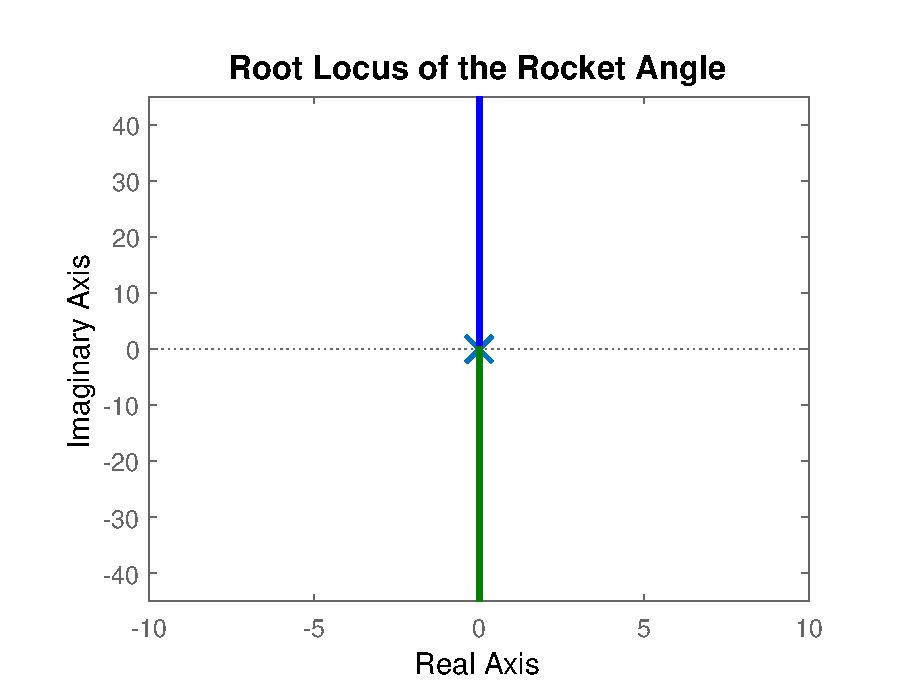
\includegraphics[width=0.7\textwidth]{figures/Rocket/design/initial_transfer_function_vf}
\caption{Root locus of the rocket angle transfer function.}
\label{fig:Rinitialtf}
\end{figure}

However the real system is also influenced by the servomotor. The transfer function of the servomotors is shown on \autoref{eq:TfServo}. 

\begin{subequations}
	\begin{flalign}
& H_s = \frac{1}{\uptau s+ 1}	\\
& H_s = \frac{1}{0.04s + 1}
\label{eq:TfServo}
	\end{flalign}
\end{subequations}
\startexplain
\explain{$\uptau$ is the time constant of the servomotors}{\si{\second}}
\stopexplain

This function then adds a pole to the initial transfer function, resulting in an unstable system. This is shown on \autoref{fig:SystemServo}.
\begin{figure}[htbp]
\centering
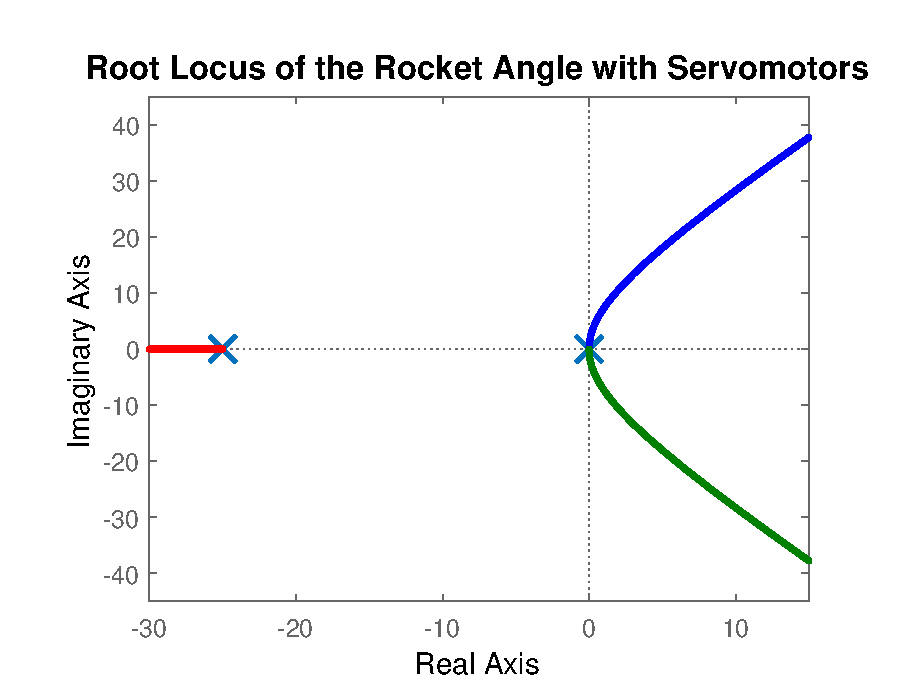
\includegraphics[width=0.7\textwidth]{figures/Rocket/design/tf_with_servo_vf}
\caption{Root locus of the system with the pole from the servomotors.}
\label{fig:SystemServo}
\end{figure}

This system could be controlled similarly to the inverted pendulum by doing cascade control. By having an inner loop that controls the servomotors as fast as possible the pole added can be assumed to have no effect. This would make the rocket control design nearly identical to the inverted pendulum by having an inner loop with a simple gain and an outer loop where a compensator in form of a zero needs to be added. 

The rocket built however doesn't have any sensors to measure the servomotors so this isn't an option. If the rocket was built differently this would be the preferred way to control it.

Instead an attempt to control the system using an inner loop.

\subsection{Controlling the Rocket Angle without Cascade Control}
To move the poles to the left half plane, a controller C1, adding a zero and a pole on the left side, is implemented to the rocket transfer function. If the zero is placed to close to the servo pole the loci will not be attracted to the real axis. Common practice recommends placing the pole at a location 20-40 times larger than the zero. Thus the zero of the controller is chosen experimentaly near the system in order to attract the poles, and the pole of the controller at a 40 times larger position. The controller C1 is shown on \autoref{eq:TfC1}.
\begin{equation}
C1 = \frac{s + 1.7}{s + 68}	\label{eq:TfC1}
\end{equation}

\begin{figure}[htbp]
\centering
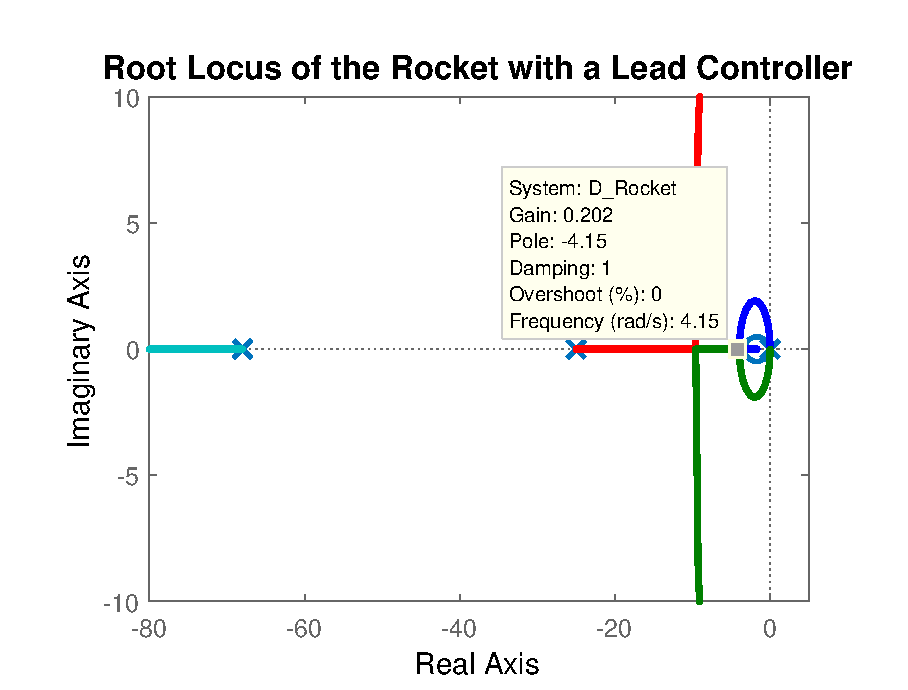
\includegraphics[width=\textwidth]{figures/Rocket/design/tf_with_controller_final_general}
\caption{Root locus of the system with a lead controller, C1, added.}
\label{fig:SystemC1}
\end{figure}

The rocket requires a fast settling time and rise time in order to act as soon as possible and control the rocket's stability. Lead compensaters enable the modulation of the rise time, but impact the overshoot. The overshoot is considered as an inferrior error, being in part countered by the play of the gimbal system. 
According to the specification the setling time should be faster than 1.5 second and the overshoot less than 25 per cent.

To improve the rise time, the gain is set at $0.404$ \si{\dB}. This value is chosen by observing the root locus and the gain of a set point, as shown on \autoref{fig:SystemC1C2Zoom}.  

				% Figure of chosen point
\begin{figure}[htbp]
	\centering
	
	\includegraphics[width=\textwidth]{figures/Rocket/design/tf_with_controller_final}
	\caption{Set point at the start of the circle.}
	\label{fig:SystemC1C2Zoom}
	
\end{figure}

To further improve the rise time and setling time of the rocket transfer function until the pysical and specification limits, the gain is doubled. 
The step response of the controlled rocket transfer function is shown on \autoref{fig:StepFinalRocket}.

\begin{figure}[htbp]
	\centering
	\includegraphics[width=\textwidth]{figures/Rocket/design/step_response_final}
	\caption{Step response of the rocket transfer function.}
	\label{fig:StepFinalRocket}
\end{figure}

The bodeplot of the controlled rocket transfer function is shown on \autoref{fig:BodePlotFinalTf}. The frequency correponds to a complete rotation of the servomotors. At low frequencies a delay is observed. However the system functions at low speed. This implies that the delay has a tempered effect on the system. Higher frequencies are not physicaly possible and do not need to be compensated.

				% Figure of final tf bodepoint
\begin{figure}[htbp]
	\centering
		\includegraphics[width=\textwidth]{figures/Rocket/design/bodeplot}
		\caption{Bodeplot of the rocket transfer function.}
		\label{fig:BodeplotFinalTf}
\end{figure}

The controlled rocket transfer function obtained is shown on equation \autoref{eq:RocketTfEqu} and  \autoref{fig:FinalChartNumbers}.

\begin{equation}    
H = 0.404 \cdot \frac{s + 1.7}{s + 68} \cdot \frac{1}{s \cdot \uptau + 1} \cdot \frac{F_t \cdot L_{Cg} \cdot \frac{1}{M_r \cdot L_{Es}^2}}{s^2}  
\end{equation}
\label{eq:RocketTfEqu}

\begin{figure}[htbp]
	\centering
	
	\includegraphics[width=\textwidth]{figures/Rocket/design/final_chart_number}
	\caption{Rocket transfer function.}
	\label{fig:FinalChartNumbers}
	
\end{figure}

%\subsection{Design of Thrust Vectoring System}
%\todo{Raphael task describe gimbal. - Mathias}

  
